\section{Исследование двумерной дискретной системы}
        \subsection{Формулировка задачи}
            Рассматривается двумерная динамическая система с дискретным временем
            \begin{equation} \label{TwoStepSystem}
                u_{t+1} = r u_t^2 e^{-u_{t-1}},\; u_t > 0,\; \forall t = 0,\; 1,\: 2,\: \dots
            \end{equation}
            при положительных значениях параметра $r$.

            В рамках задачи для системы \ref{TwoStepSystem} требуется:
            \begin{enumerate}
                \item
                    найти неподвижные точки;
                \item
                    исследовать на устойчивость найденные неподвижные точки в зависимости от параметра $r$;
                \item
                    исследовать вопрос возникновения бифуркации Неймарка-Сакера, построить инвариантную кривую в соответствующем случае.
            \end{enumerate}
        \subsection{Поиск неподвижных точек}
            \begin{definition}
                Точка $u^*\in\R$ называется неподвижной точкой системы $u_{t+1}=f(u_t,u_{t-1}),\; u_t\in\R,\; f:\R^2\rightarrow\R$, если $u^* = f(u^*,u^*)$.
            \end{definition}

            Для поиска неподвижных точек необходимо решить уравнение
            $$
                u^* = r (u^*)^2 e^{-u^*},
            $$
            которое полностью совпадает с уравнением \ref{OneStepFind}, рассмотренным ранее. Поэтому запишем вывод из предыдущего пункта:
            \begin{enumerate}
                \item
                $0 < r < e$:
                $$u^* = 0.$$
                \item
                $r = e$:
                $$u^*_1 = 0, \; u^*_2 = 1.$$
                \item
                $r > e$:
                $$u^*_1 = 0, \; u^*_2 \in (0, 1), \; u^*_3 \in (1, +\infty).$$
            \end{enumerate}
        \subsection{Исследование неподвижных точек на устойчивость}

            Рассмотрим динамическую систему \ref{TwoStepSystem}. Пусть $v_t = u_{t-1}$, тогда
            \begin{equation}\label{TwoStepBigSystem}
                \left\{
                    \begin{array}{ll}
                        u_{t+1} = r u^2_t e^{-v_t},\; r > 0,\; u_t > 0,\; v_t > 0 \\
                        v_{t+1} = u_t.
                    \end{array}
                \right.
            \end{equation}
            \begin{theorem}\label{th:yakobi}
                Пусть дана динамическая система с дискретным временем $u_{t+1}=f(u_t),\;u_t\in\R^n,\;t\in\N$, $f$~--- гладкое отображение, $\R^n\rightarrow\R^n$. Тогда неподвижная точка $u^*$ асимптотически устойчива, если все собственные значения $\lambda_1,\;\lambda_2,\;\ldots,\;\lambda_n$ матрицы Якоби функции $f(u)$ в точке $u^*$ удовлетворяют условию $|\lambda_i|<1,\;i = 1,\;2,\;\ldots,\;n$. Если модуль хотя бы одного собственного значения больше единицы, то $u^*$ неустойчива.
            \end{theorem}

            Чтобы воспользоваться теоремой \ref{th:yakobi}, выпишем матрицу Якоби системы \ref{TwoStepBigSystem}:

            $$
                J(u, v)
                = 
                \begin{pmatrix}
                        \frac{\partial f_1}{\partial u} &
                        \frac{\partial f_1}{\partial v} \\
                        \frac{\partial f_2}{\partial u} &
                        \frac{\partial f_2}{\partial v} 
                \end{pmatrix}
                =
                \begin{pmatrix}
                        2rue^{-v}
                        & 
                        -ru^2e^{-v}
                        \\
                        1
                        &
                        0 
                \end{pmatrix}.
            $$

            Рассмотрим точку $u^* = 0$. 
            $$
                J(u^*)=
                \begin{pmatrix}
                    0 & 0 \\
                    1 & 0
                \end{pmatrix}
            $$
            Матрица Якоби имеет одно собственное значение $\lambda_{1, 2} = 0$. Очевидно, что эта точка асимптотически устойчива, причем для любого значения $r$.

            Рассмотрим $r = e$ и неподвижную точку $u^* = 1$.
            $$
                J(u^*)=
                \begin{pmatrix}
                    2 & -1 \\
                    1 & 0
                \end{pmatrix}
            $$
            Матрица Якоби имеет одно собственное значение $\lambda_{1, 2} = 1$. Поэтому об устойчивости этой точки ничего сказать нельзя.

            Рассмотрим $r > e$ и неподвижные точки $u^*_1 \in (0, 1)$ и $u^*_2 \in (1, +\infty)$.
            Так как эти точки удовлетворяют соотношению $u^*e^{-u^*} = \frac{1}{r}$, xарактеристический многочлен матрицы Якоби принимает вид
            $$
                |J(u^*) - \lambda I|
                =
                -\lambda(2 - \lambda) + u
                =
                \lambda^2 - 2\lambda + u.
            $$
            В таком случае,
            $$
                \lambda_{1, 2}
                =
                \frac{2 \pm \sqrt{4 - 4u}}{2}
                =
                1 \pm \sqrt{1 - u}.
            $$
            Получается, что $u^*_1$ и $u^*_2$ неустойчивы.

\begin{figure}[h]
        \centering
        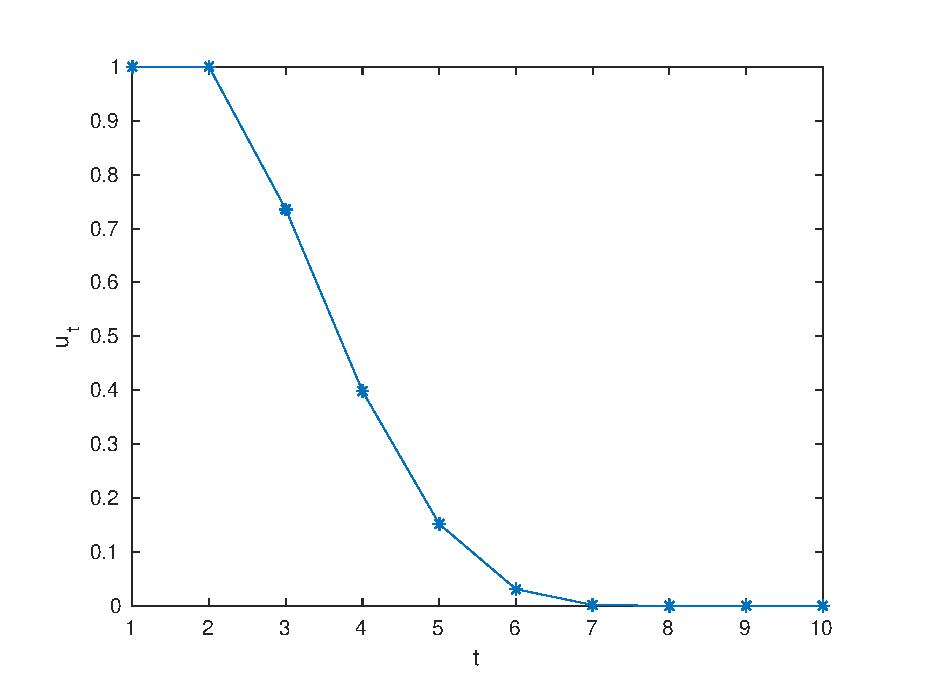
\includegraphics[width=0.8\linewidth]{second_discrete_system/stability_r2.eps}
        \caption{Орбита системы \ref{TwoStepSystem} при $r = 2,\; u_0 = u_1 = 1$.}
\end{figure}
\begin{figure}[h]
        \centering
        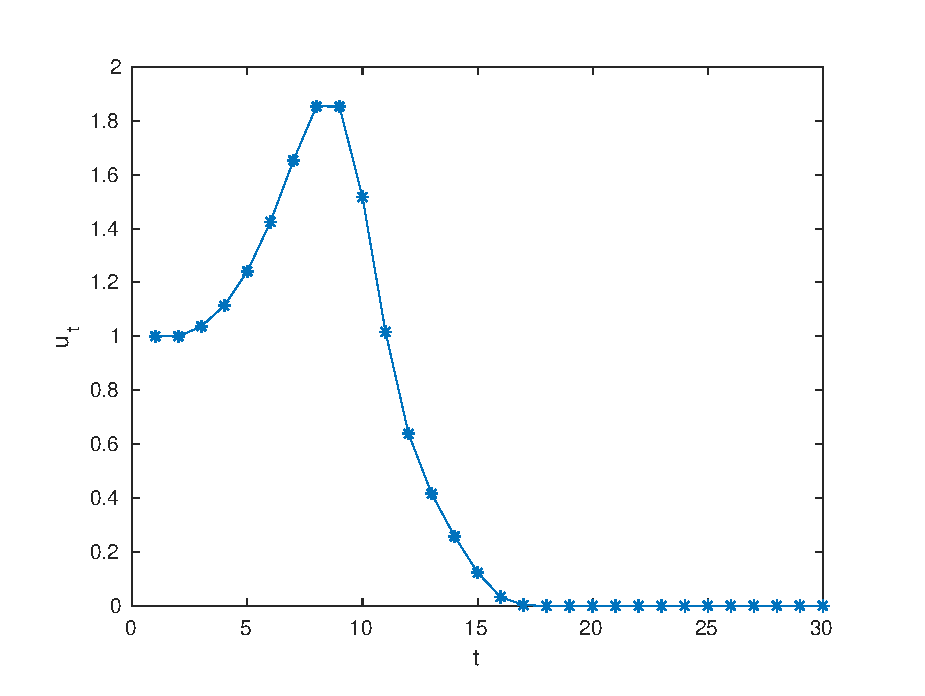
\includegraphics[width=0.8\linewidth]{second_discrete_system/stability_replus0-1.eps}
        \caption{Орбита системы \ref{TwoStepSystem} при $r = e + \frac{1}{10},\; u_0 = u_1 = 1$.}
\end{figure}

        \subsection{Бифуркация Неймарка-Сакера}
            \begin{definition}
                Бифуркация положения равновесия в системе \ref{TwoStepSystem}, соответствующая появлению мультипликаторов $|\lambda_1| = |\lambda_2| = 1,\;\lambda_1 = \overline{\lambda_2}$, называется бифуркацией Неймарка-Сакера или дискретной бифуркацией Хопфа. \cite[стр.~252]{bratus10}
            \end{definition}

            Из предыдущего пункта мы получили, что при $r = e,\; u^* = 1$ возникает бифуркация Неймарка-Сакера. При $r > e$ в окрестности $u^* = 1$ появляются две неустойчивые неподвижные точки. При $r < e$ неподвижной точки не сущствует в принципе.
            \begin{figure}[h!]
                \centering
                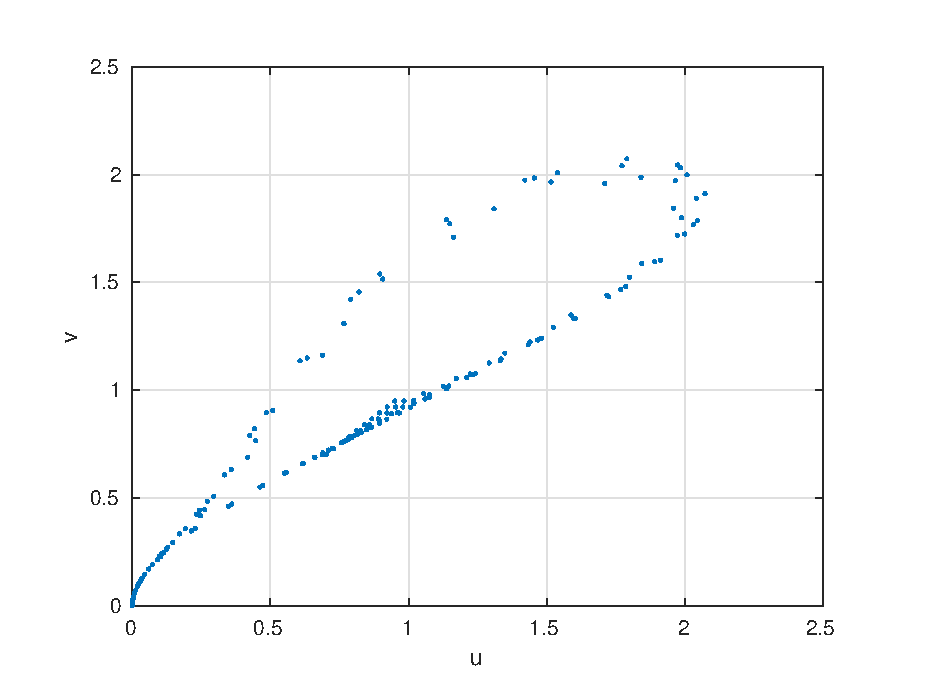
\includegraphics[width=0.8\linewidth]{img/two_step_bifurcation_gt.eps}
                \caption{Поведение системы \ref{TwoStepSystem} в окрестности точки $(1, 1)$ при $r = e + \frac{1}{10}$.}
                \label{img:two_step_bifurcation_gt}
            \end{figure}
                        \begin{figure}[h!]
                \centering
                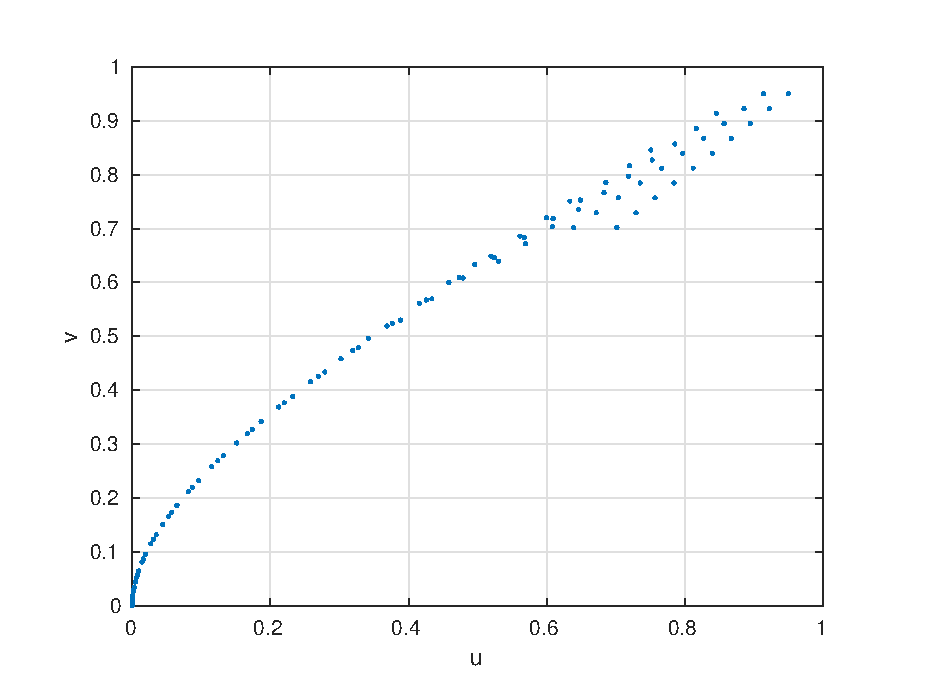
\includegraphics[width=0.8\linewidth]{img/two_step_bifurcation_lt.eps}
                \caption{Поведение системы \ref{TwoStepSystem} в окрестности точки $(1, 1)$ при $r = e - \frac{1}{10}$.}
                \label{img:two_step_bifurcation_lt}
            \end{figure}